\section{Data pipeline}
In this section we'll discuss the processing steps we applied to the data, after retrieving it and converting it to a
useful format. This goes in addition to any steps taken in the previous section. 

\subsubsection{What features to focus on}
For the models, we chose to primarily focus on the content of the articles as predictors for whether a given article is
fake or not. Whilst we were tempted to include "domain" initially, after the discovery discussed in section \ref{sec:truth_pr_domain},
we decided against We also chose to ignore the titles of the articles, as these where often simply reflections of the
content.

\subsubsection{Grouping}
Whilst it is possible to use logistic regression for multi-class classification, we instead chose to build a binary
classifier, that tries to establish wether an article is "reliable" or not. Because of our focus on the reliability of
the article, we chose to encode all "reliable" articles as 1's, whilst the rest of the types ("fake", "bias", etc.) got
encoded as 0's. With this approach we will be (perhaps unfairly) strict in our judgement of a given article, but we
reason that it is better to accidentally label a reliable article as false, than it is to accidentally label a false
article as reliable. \todo{Maybe we should include an appendix with alternative model results for hard classification of
fake news?}

\subsubsection{Splitting the dataset}
At this point we start moving into territory where we need to split our data. So we decided to split our data into into
a training, validation and testing set, with a 80-10-10 split.

\subsubsection{Tokenization}
After filtering out duplicate articles \ref{sec:dup_articles} and deciding to focus on the content of
the articles for our input, the next step was to tokenize the data. We tokenized the text by first splitting it into
individual words, removing stop words and using lemmitization to further reduce the vocabulary by condensing words into
base form.

\subsubsection{Feature extraction using TF-IDF}
After treated the content column, we were then able to train a TF-IDF (Term Frequency - Inverse Document Frequency)
model on it. This model looks at how often a given token (word) appears in an article, and compares it to how big that
document is. By training this model, we essentially output a large vector, which we can use to encode the tokens into a
large matrix that can be fed into our models.

\subsubsection{Dimensionality reduction using Truncated Single Value Decomposition (SVD)}
After encoding the data using our TF-IDF model, we were left with quite a large input space, which meant that it would
be useful for us to reduce the dimensionality of our input matrix. In other words, we wanted to group similar elements
(or flags) together, such that the models we build have a more clear delineation between inputs. To this we used
truncated single value decomposition (SVD), that works by factoring a matrix with the hopes to extract most impactful
elements of it.

\subsubsection{Individual model differences}
Whilst the above steps are broadly applicable to all the models we built, there was some individual differences on what
steps and what hyperparameters each model was built with. These are seen in figure \ref{fig:pipeline}.

\begin{figure}[htpb]
  \centering
  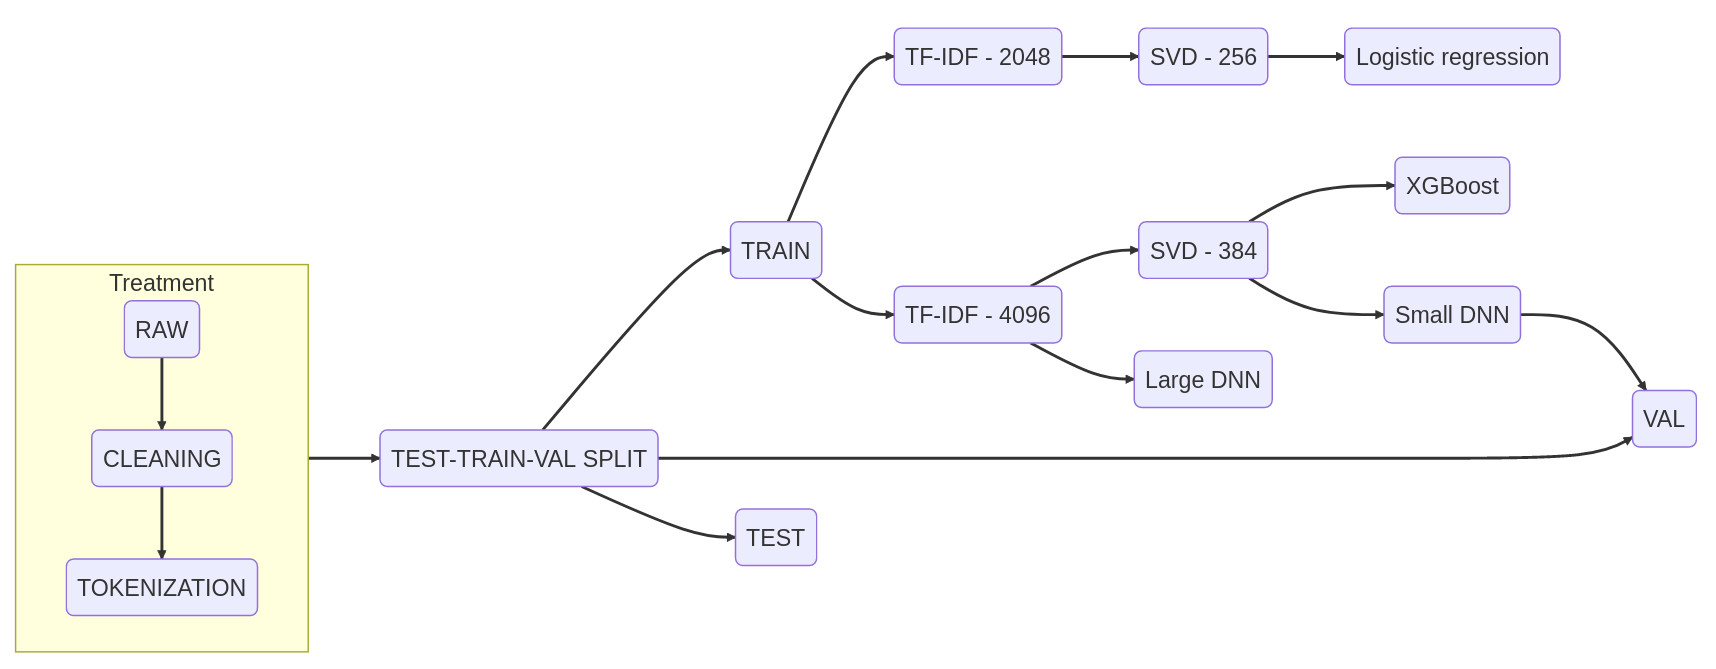
\includegraphics[width=1\textwidth]{pipeline}
  \caption{Pipeline}
  \label{fig:pipeline}
\end{figure}

There were a few reasons for the differences:
\begin{enumerate}
  \item \textbf{Logistic regression}: For our simple model we initially set the TF-IDF and SVD parameters quite low. We
    set our TF-IDF model to output a 2048 dimensional vector that get reduced to 256 dimensions through SVD.

  \item \textbf{XGBoost and baseline DNN}: We suspected that the smaller dimensionality of our simple model, might
    impact our results negatively, and since the models were fairly straight forward to train we choose to increase the
    dimensionality such that our TF-IDF ouputted a 4096 dimensional vector, that then got reduced to 384 dimensions.

  \item \textbf{Alternative DNN} : Lastly chose to omit the dimensionality reduction from the alternative (large DNN),
    in ordet to see wether a larger model would improve performance.
\end{enumerate}
